\documentclass{article}
\usepackage{tikz}
\usepackage{graphicx}
\usepackage{tikz}
\usepackage{graphicx}
\usepackage{amsmath}
\usepackage{bm} 

\begin{document}

\begin{figure}[h]
\begin{center}
\begin{tikzpicture}
    % imagen
    \node[inner sep=0] (image) at (0,0) 
          {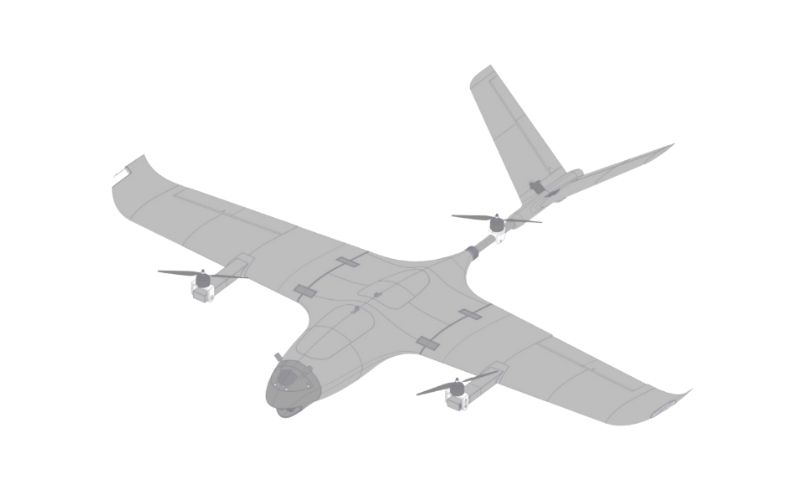
\includegraphics[width=15cm]{fbd.png}};

    %ejes pitch yaw roll
    \draw[dashed, black!60] (-3,-3.45) -- (4,2);
    \draw[dashed, black!60] (-5.5,1.5) -- (5.5,-3.25);
    \draw[dashed, black!60] (0.2,3) -- (0.2,-4);

    % gravedad
    \draw[-latex, ultra thick, green!50!black] (0.2,-0.95) -- (0.2,-2.2);
    \node at (-0.3,-2.15) {$mg^{I}$};

    % marco b
    \draw[-latex, ultra thick] (0.2,-0.95) -- (0.2,1.15);
    \draw[-latex, ultra thick] (0.2,-0.95) -- (-1.5,-2.28);
    \draw[-latex, ultra thick] (0.2,-0.95) -- (2.25,-1.85);

    % marco i
    \draw[-latex, ultra thick] (-8,-3) -- (-8,-1.5);
    \node[font=\small] at (-8,-1.2) {${{z}^{I}}$};
    \draw[-latex, ultra thick] (-8,-3) -- (-8.8,-3.75);
    \node[font=\small] at (-9,-4) {${{y}^{I}}$};
    \draw[-latex, ultra thick] (-8,-3) -- (-6.5,-3);
    \node[font=\small] at (-6.25,-3) {${{x}^{I}}$};

    % momentos pitch yaw roll
    \draw[<->, ultra thick] (0.125,2.85) arc (95:435:0.5cm and 0.25cm);
    \node[font=\Large] at (0.125,3.5) {${\tau_{z}^{b}}$};
    \draw[<->, ultra thick] (5.7,-3.25) arc (0:340:0.25cm and 0.5cm);
    \node[font=\Large] at (6.15,-3.5) {${\tau_{y}^{b}}$};
    \draw[rotate=10, <->, ultra thick] (-3.75,-3) arc (180:500:0.25cm and 0.5cm);
    \node[font=\Large] at (-3.75,-3.75) {${\tau_{x}^{b}}$};

    % fuerzas L y D cola - standardized to 1.25 length
    \draw[-latex, ultra thick, blue!70!black] (2.2,2.35) -- ++(0.4,0.96);
    \node at (2.8,3.45) {${L_{6}}$};
    \draw[-latex, ultra thick, blue!70!black] (2.2,2.35) -- ++(0.8,0.65);
    \node at (3.15,3.15) {${D_{6}}$};
    \draw[-latex, ultra thick, blue!70!black] (4.15,1.65) -- ++(-0.32,0.88);
    \node at (3.65,2.65) {${L_{5}}$};
    \draw[-latex, ultra thick, blue!70!black] (4.15,1.65) -- ++(0.56,0.56);
    \node at (4.85,2.35) {${D_{5}}$};

    % fuerzas L y D alerones - standardized to 1.25 length
    \draw[-latex, ultra thick, blue!70!black] (-3.15,0.75) -- ++(0,1.25);
    \node at (-2.85,2.15) {${L_{3}}$};
    \draw[-latex, ultra thick, blue!70!black] (-3.15,0.75) -- ++(0.9,0.75);
    \node at (-2.1,1.65) {${D_{3}}$};
    
    \draw[-latex, ultra thick, blue!70!black] (3.45,-2.1) -- ++(0,1.25);
    \node at (3.65,-0.7) {${L_{2}}$};
    \draw[-latex, ultra thick, blue!70!black] (3.45,-2.1) -- ++(0.85,0.7);
    \node at (4.45,-1.25) {${D_{2}}$};

    % fuerzas L y D alas - standardized to 1.25 length
    \draw[-latex, ultra thick, blue!70!black] (-4.65,0.95) -- ++(0,1.25);
    \node at (-4.45,2.35) {${L_{4}}$};
    \draw[-latex, ultra thick, blue!70!black] (-4.65,0.95) -- ++(0.8,0.7);
    \node at (-3.7,1.8) {${D_{4}}$};
    
    \draw[-latex, ultra thick, blue!70!black] (4.25,-2.85) -- ++(0,1.25);
    \node at (4.45,-1.45) {${L_{1}}$};
    \draw[-latex, ultra thick, blue!70!black] (4.25,-2.85) -- ++(0.75,0.7);
    \node at (5.15,-2.35) {${D_{1}}$};
    
    % ángulos gamma
    \draw[dashed, thick, red!80] (2.2,2.35) -- (2.85,3.5);
    \draw[rotate=-45, ultra thick, red] (0.1,3.45) arc (40:120:0.25cm and 0.75cm);
    \node at (3,3.75) {${\gamma_{2}}$};
    \draw[dashed, thick, red!80] (4.15,1.7) -- (3.5,3);
    \draw[ultra thick, red] (4.35,1.7) arc (40:120:0.25cm and 0.75cm);
    \node at (3.5,3.15) {${\gamma_{1}}$};

    % ángulos epsilon
    \draw[dashed, thick, red!80] (-4.70,-1.5) -- (-3.75,-0.85);
    \draw[ultra thick, red] (-4.3,-1.25) arc (210:90:0.7cm and 1cm);
    \node[font=\large] at (-4.85,-1.75) {${\epsilon_{2}}$};
    \draw[dashed, thick, red!80] (1,-2.9) -- (-0.05,-3.75);
    \draw[ultra thick, red] (0.45,-3.3) arc (210:90:0.7cm and 1cm);
    \node[font=\large] at (-0.25,-4) {${\epsilon_{1}}$};
    
    % momentos M
    \draw[-latex, ultra thick, blue!60] (-3.2,-0.25) arc (0:-270:0.5cm and 0.25cm);
    \node at (-3,-0.75) {${\tau_{2}}$};
    \draw[-latex, ultra thick, blue!60] (1.55,-2.3) arc (0:270:0.5cm and 0.25cm); 
    \node at (1.75,-2.8) {${\tau_{1}}$};
    \draw[-latex, ultra thick, blue!60] (2.3,0.8) arc (0:-270:0.5cm and 0.25cm);
    \node at (2.25,0.25) {${\tau_{3}}$};

    % fuerzas M - standardized to 1.25 length
    \draw[-latex, ultra thick, blue!70!black] (-3.70,-0.3) -- ++(0,1.25);
    \node at (-3.5,1.1) {${f_{2}}$};
    \draw[-latex, ultra thick, blue!70!black] (1.075,-2.25) -- ++(0,1.25);
    \node at (1.3,-0.85) {${f_{1}}$};
    \draw[-latex, ultra thick, blue!70!black] (1.825,0.75) -- ++(0,1.25); 
    \node at (2.05,2.15) {${f_{3}}$};

    % ángulo de ataque
    \draw[dashed, thick, red!50!black] (0.2,-0.95) -- (-1.5,-1);
    \node[red!50!black] at (-1.5,-0.65) {$\hat{V}_{rel}$};
    \draw[ultra thick, red!50!black] (-0.5,-1.5) arc (210:180:0.7cm and 1cm);
    \node at (-0.85,-1.35) {${\alpha}$};
    
\end{tikzpicture}
\end{center}
\end{figure}

\end{document}